\part{Deep Learning}
\chapter{General}

\section{Techniques for uncertainties (old)}

\subsection{Dropout}
The dropout method has been used for a long time in order to avoid over-fitting. Networks nodes (i.e. neurons) are disable randomly during training time so that with each training step, a different subset of the network architecture is evaluated and adjusted. This can be seen as a regularization and proves to result in better generalization in many cases.

\subsection{Dropout and scaling}
Setting a dropout rate greater than 0, will change the magnitude of the values passed through the network. Consider a simple example of two layers of size 10 and 1. If all activations are approximately 1, the output should be around 10. Now, if we add a dropout with rate 0.5, the output will be around 5. This means that the activation will be too big at test time and need to be rescaled. To avoid an additional operation at test time, this is done at training time with a scaling factor of $\frac{1}{1-p}$.


\subsection{Dropout Sampling (Monte-Carlo)}
Randomly turns off network node during inference. This results in a random prediction with some complex probability distributions every time an input value is passed to the network. The empirical distribution or parameter estimates can be used to obtain, for example, a mean value and a confidence measure in terms of the distributional variance. We expect that the empirical variance is low here there was an abundance of training data since all network subsets had the opportunity to learn in these areas. However, in areas where there was no training data to learn from, the network behavior is not controllable so we expect a high variance among the different network subsets.


\subsection{Deep Ensembles}
in a general regression setup, the neural network takes a vector of inputs and generates a single output that represents our prediction. This is done according the network parameters obtained during training process. However ,if we assume our real data to behave according to a parametric probability distribution whose parameters depend on the input values, we can take the underlying model into account and estimate not only the actual output value but a set of distributional parameters.

Assume that our model has a single output $y$ which is not deterministic but normally distributed with parameters $(\mu(x), \sigma^2(x)$ depending on the input $x$. In the training, instead of using the common mean squared error loss function, we will take into account the distribution as well. We can achieve this by using a maximum likelihood (ML) approach. We can take the negative log-likelihood function of the normal distribution as a loss function (ignoring the constants).

\begin{equation}
    \mathcal{L}(x, y) = -log \phi(y|x) = \frac{log \hat{\sigma}^2(x)}{2}+\frac{(y-\hat{\mu}(x))^2}{2\hat{\sigma}^2(x)}
\end{equation}

And for multiple samples, we average to minimize the \textit{mean negative log-likelihood}.
intuitively, the numerator of the right term encourages the mean prediction $\hat{\mu}(x)$ to be close to the observed value. The denominator term ensures that the variance $\hat{\sigma}^2(x)$ is large when the mean prediction is far from the observed data.

\subsection{Ensemble Averaging}

Instead of training a single network, the idea is to train an ensemble of $M$ networks with different initialization. We expect that all the networks behave similarly in areas with sufficient training data and give completely different results where there is no data available.
For the final prediction, they combine all the results of the networks into a Gaussian mixture distribution, from which it is possible to extract a single mean and variances estimations.

\subsection{Dropout Ensembles}
Combine Dropout and Deep Ensembles.

\subsection{Quantile Regression}
Another classic method for distribution estimation with neural networks.

\subsection{Gaussian Process}
A Gaussian Process is a random function that is defined by its mean and covariance functions.

\section{Bayesian Deep Learning}

\subsection{Two kind of uncertainties}
In Bayesian modeling, there are two main kinds of uncertainties that we can model: \textit{epistemic} and \textit{aleatoric} uncertainty.

\paragraph{Epistemic uncertainty} accounts for uncertainty in the model parameters which captures the ignorance of the model for a certain input data. This uncertainty can be reduced if more training data are given.

\paragraph{Aleatoric uncertainty} captures the noise in the input data, for example, sensor noise. This type of noise cannot be reduced even if more data were collected.
Aleatoric uncertainty can further be categorized into:
\begin{itemize}
    \item \textit{homoscedastic uncertainty}, uncertainty which stays constant for different inputs
    \item \textit{heteroscedastic uncertainty}, uncertainty which depends on the input data
\end{itemize}

\subsection{Weight Uncertainty in Neural Networks}
\subsubsection{Terminology}

\begin{equation}
    P(\mathbf{w}|\mathcal{D}) = \frac{P(\mathcal{D}|\mathbf{w})P(\mathbf{w})}{P(\mathcal{D})} = \frac{P(\mathcal{D}|\mathbf{w})P(\mathbf{w})}{\int P(\mathcal{D}|\mathbf{w})P(\mathbf{w}) d\mathbf{w}}
\end{equation}

\begin{itemize}
    \item $\mathbf{w}$ are the weights of the network.
 \item $\mathcal{D}$ is the training data.
\item $P(\mathbf{w}|\mathcal{D})$ is the \textbf{posterior} probability of $\mathbf{w}$. This is the probability distribution of the weights given an observed set of data.
\item $P(\mathcal{D}|\mathbf{w})$ is the \textbf{likelihood} of $\mathbf{w}$. This is the probability distribution of the data given fixed weights.
\item $P(\mathbf{w})$ is the \textbf{prior} probability on $\mathbf{w}$. This represents our initial beliefs on the distribution of the weights, before observing any data.
\item $P(\mathcal{D})$ is the \textbf{evidence} (also called marginal likelihood) of the data.
\end{itemize}


Log-probabilities are often used instead because they provide better numerical stability. Probabilities are usually small numbers and multiplication of them can be imprecise. Taking the log gives large negative values and transforms products into additions.


\subsubsection{Bayesian Inference and Prediction}

A neural network can be viewed as a probabilistic model $P(y|x, \mathbf{w})$. In case of classification, this corresponds to the softmax output.

The normal approach of training a neural network by updating weights using gradient descent seeks to find the weights which best explain the data. This can be seen as learning the weights which maximize the likelihood $P(\mathcal{D}|\mathbf{w})$, through \textbf{Maximum Likelihood Estimation (MLE)}.

\begin{align}
    \mathbf{w}^{MLE} &= \arg\max_{\mathbf{w}} P(\mathcal{D}|\mathbf{w}) \\
    & = \arg\max_{\mathbf{w}} \prod_i P(y_i|x_i, \mathbf{w})
\end{align}

This is the frequentist perspective, where the weights are fixed and the data is viewed as a random variable. 
Instead, we can view the data as being fixed and the model weights as being a random variable. We can train to maximize the posterior $P(\mathbf{w}|\mathcal{D})$ via \textbf{Maximum a Posteriori (MAP)} learning. This is equivalent to MLE objective  with an additional regularization term using the prior distribution of the weights:

\begin{align}
    \mathbf{w}^{MAP} &= \arg\max_{\mathbf{w}} P(\mathbf{w}|\mathcal{D}) \\
    & = \arg\max_{\mathbf{w}} P(\mathcal{D}|\mathbf{w})P(\mathbf{w}) \\
    & = \arg\max_{\mathbf{w}} \log P(\mathcal{D}|\mathbf{w}) + \log P(\mathbf{w})
\end{align}

Having obtained the MLE or MAP weights, prediction can be simply using the model with the learned weights fixed:

\begin{equation}
    P(\hat{y}|\hat{x}) = P(\hat{y}|\hat{x}, \mathbf{w}^{MLE})
\end{equation}


If we consider the entire posterior distribution of the weights $P(\mathbf{w}|\mathcal{D})$, the predictive distribution becomes a weighted expectation over all possible values for $\mathbf{w}$.

\begin{align}
    P(\hat{y}|\hat{x}) & = \mathbb{E}_{p(\mathbf{w}|\mathcal{D})}[P(\hat{y}|\hat{x}, \mathbf{w})] \\
    & = \int P(\hat{y}|\hat{x}, \mathbf{w})P(\mathbf{w}|\mathcal{D}) d\mathbf{w}
\end{align}

\subsubsection{Variational Inference}
Unfortunately, this predictive distribution is generally intractable for neural networks. Also, even if the prior $P(\mathbf{w})$ is something that we can choose and the likelihood $P(\mathcal{D}|\mathbf{w})$ can be computed, the posterior $P(\mathbf{w}|\mathcal{D})$ is intractable. More precisely, the evidence $P(\mathcal{D})$ in the denominator requires integration over the very high-dimensional space of weights and has no analytical solution:

\begin{align}
    P(\mathcal{D}) & = \int P(\mathcal{D}, \mathbf{w}) d\mathbf{w} \\
    & = \int P(\mathcal{D}|\mathbf{w}) P(\mathbf{w}) d\mathbf{w}
\end{align}


Thus, we need to employ approximations. \textbf{Variational inference} constructs a new distribution $q(\mathbf{w}|\theta)$ over the weights $\mathbf{w}$ and parameterized by $\theta$, that approximates the true posterior $P(\mathbf{w}|\mathcal{D})$. It finds the parameters $\theta$ which minimizes the \textit{KL}-divergence between $q$ and $P$.
\begin{equation}
    \theta^* = \arg\min_{\theta}KL[q(\mathbf{w}|\theta) || P(\mathbf{w}|\mathcal{D}]
\end{equation}

The KL-divergence is an information-theoric measure of the difference between distributions. This is not a true distance metric because it is not symmetric.

\begin{equation}
    KL[q(x)||P(x)] = \int q(x) \log \frac{q(x)}{P(x)}dx
\end{equation}

We substitute this into the previous equation and reformulat it to only depend on values we know:

\begin{align}
    \theta^* &= \arg\min_{\theta} \int q(\mathbf{w}|\theta) \log \frac{q(\mathbf{w}|\theta)}{P(\mathbf{w}|\mathcal{D})}d\mathbf{w} \\
    &= \arg\min_{\theta} \int q(\mathbf{w}|\theta) \log \frac{q(\mathbf{w}|\theta)}{P(\mathcal{D}|\mathbf{w})P(\mathbf{w})} d\mathbf{w}
\end{align}

Directly from this, we can construct a cost function which will seek the minimum setting of $\theta$ for:

\begin{align}
    \mathcal{F}(\mathcal{D}, \theta) &= \int q(\mathbf{w}|\theta) \log \frac{q(\mathbf{w}|\theta)}{P(\mathbf{w})} - q(\mathbf{w}|\theta)\log P(\mathcal{D}|\mathbf{w})d\mathbf{w} \\
    &= KL[q(\mathbf{w}|\theta)||P(\mathbf{w})] - \mathbb{E}_{q(\mathbf{w}|\theta)}[\log P(\mathcal{D}|\mathbf{w})]
\end{align}

This cost is a balance between having a variational posterior that is close tho the prior and also be able to explain the complexity of the data. The negative of this cost $-F$ is also called \textbf{Evidence Lower Bound (ELBO)}. Thus minimizing this cost function is equivalent to maximizing the ELBO. It's important to note that the variational inference is known to underestimate the uncertainty of models.


\subsubsection{Bayes by Backprop}

Calculting the expectation of the likelihood over the variational posterior is computationally prohibitive. Once more, we need to use approximation. We approximate our cost function using sampled weights:

\begin{equation}
    \mathcal{F}(\mathcal{D}, \theta) \approx \sum_{i=1}^n \log q(\mathbf{w}^{(i)}|\theta) - \log P(\mathbf{w}^{(i)}) - \log P(\mathcal{D}|\mathbf{w}^{(i)})
\end{equation} 

Using automatic differentiation as provided by frameworks such as PyTorch, we only need to worry about implementing this sampling, and setting up the cost function as above. The usual backpropagation methods can be used to train the model.


\section{Recent architectures}

\subsection{Components}

\paragraph{Convolutions} A convolution layer is composed of a set of convolutional kernels. Each kernel is applied through a convolution to a small block of the image, named the receptive field.


\paragraph{Pooling} Feature motifs, which result as an output of convolution operation, can occur at different locations in the image. Once features are extracted, its exact location becomes less important as long as its approximate position relative to others is preserved. Pooling or down-sampling is an interesting local operation. It sums up similar information in the neighborhood of the receptive field and outputs the dominant response within this local region.
The use of pooling operation helps to extract a combination of features, which are invariant to translational shifts and small distortions

\paragraph{Activation functions} serve as a decision function and the selection of an appropriate activation function can accelerate the learning process. Usually ReLU is a good choice.

\paragraph{Batch Normalization} is used to address the issues related to the internal covariance shift within feature-maps. The internal covariance shift is a change in the distribution of hidden units' values, which slows down the convergence and requires careful initialization of parameters. BN unifies the distribution of feature-map values by setting them to \textbf{zero mean} and \textbf{unit variance}. Furthermore, it smoothens the flow of gradient and acts as a regularization factor, which helps generalization.

\paragraph{Dropout} introduces regularization within the network by randomly skipping some units. This random dropping of some connections or units produces several thinned network architectures, and finally, one representative network is selected with small weights.This selected architecture is then considered as an approximation of all of the proposed networks.

\paragraph{Fully connected layers} is mostly used at the end of the network. It is a global operation, which globally analyzes the output of the preceding layers. It makes a non-linear combination of selected features.

% IMAGES 

CNN architectures can be broadly categorized into 7 classes:
\begin{enumerate}
    \item Spatial Exploitation: where convolutions of different sizes were compared
    \item Depth based: deeper networks seemed to learn more information
    \item Multi-path: 
    
    \item Width based:
    
    \item Feature-map Exploitation
    
    \item Channel Boosting
    
    
    \item Attention based
\end{enumerate}{}

\subsubsection{Spatial Exploitation}
As convolutional operation considers the neighborhood (locality) of input pixels, therefore different levels of correlation can be explored by using different filter sizes. Different sizes of filters encapsulate different levels of granularity; usually, small size filters extract fine-grained and large size extract coarse-grained information.
Different studies suggested that CNN can perform well both on coarse and fine-grained details.

\textbf{Exemples}: LeNet, AlexNet, ZfNet, VGG, GoogleNet

\subsubsection{Depth based}
Deep CNN architectures are based on the assumption that with the increase in depth, the network can better approximate the target function with a number of nonlinear mappings and more enriched feature hierarchies.

\textbf{Exemples}: ResNet, Highway Networks, Inception-V3, Inception-V4 and Inception-ResNet

\subsubsection{Multi-path}
Training a deep network is a challenging task because they may suffer from performance degradation, gradient vanishing or explosion problems, which are not caused by overfitting but instead by an increase in the depth. Multiple paths or shortcut connections can systematically connect one layer to another by skipping some intermediate layers to allow specialized flow of information across the layers. These path s also try to solve the vanishing gradient problem by making gradient accessible to lower layers. Different types of shortcut connections exist: zero-padded projection-based, skip connections, 1x1 connections, ...

\textbf{Exemples}: ResNet, Highway Networks, DenseNet, ... 

\paragraph{ResNet}
ResNet is composed of residual blocks that can consist of several hidden units. The input of the block goes through a second path and is usually added just before the last activation function (see figure \label{fig:resnet}).
Learning is thus based on a residual information. ResNet suggested that residual functions are easier to optimize.

Compared to Highway Network, these connections are data-independent and parameter-free.

\begin{figure}[H]
    \centering
    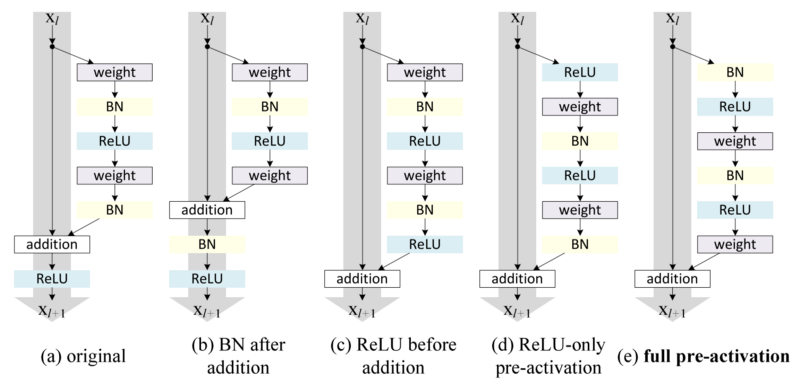
\includegraphics[scale=0.3]{content/resnet.png}
    \caption{Residual block of a ResNet}
    \label{fig:resnet}
\end{figure}

\paragraph{DenseNet}
also tried to solve the vanishing gradient problem. The problem with ResNet is that it explicitly preserves information through the additive identity transformation of the second path of the block. Thus many layers may contribute very little. The idea of DenseNet is to connect each preceeding layer to the next coming layer by concatenation. With this, the network may gain the ability to differentiate between information that is added to the network and information that is preserved. However, due to its structure, DenseNet is quite expensive in term of parameters. 
Apparently, because each layer has a direct access to gradient through the loss function, it acts as a regularization and reduces overfitting on tasks with smaller training sets.


\subsubsection{Width based}
After the trend of very deep network, some studies also reported that the width of the network as also important. One major problem of deep architectures is that some layers may not learn useful features. To tackle this problem, the focus shifted from deep and narrow architectures towards thin and wide architectures.

\textbf{Exemples}: Wide ResNet, Pyramidal Net, Xception, ...

\subsubsection{Feature-Map (Channel) exploitation}
In CNN, features are dynamically selected  by tuning the weights associated with a kernel (mask). However, some of the feature-maps can have a very little or no role in object discrimination. Enormous feature sets may create an effect of noise and thus lead to over-fitting of the network.
Here, they suggest that a good selection of feature-maps can play an important role in improving the generalization of the network.

\paragraph{Sequeeze and excitation Networks}
Teh squeeze block generates feature-map-wise statistics by suppressing the spatial infromation. Then, excitation operation assigns weights to the feature-maps.

\begin{figure}[H]
    \centering
    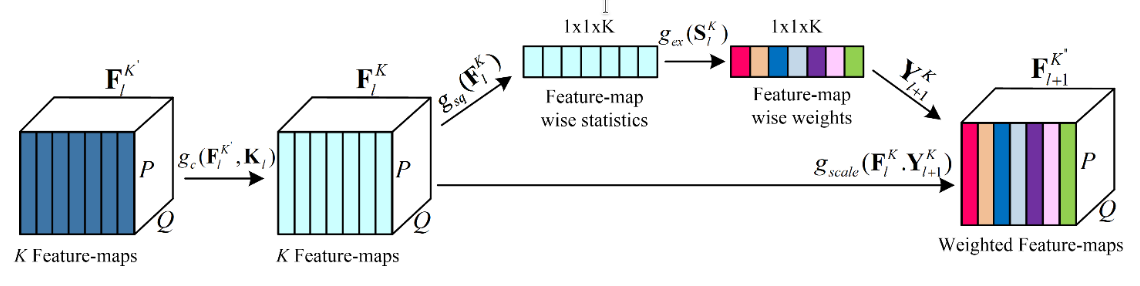
\includegraphics[scale=0.3]{content/squeeze_excitation.png}
    \caption{Squeeze and Excitation for feature-maps selection}
    \label{fig:squeeze_excitation}
\end{figure}


\subsubsection{Channel Boosting}
Image representation plays an important role in determining the performance of an algorithm. The learning of a CNN relies in this input representation and the lack of diversity and the absence of class discernable information may affect its performance.
Channel boosting of adding some extra channels (known as auxiliary channels) to the input data. The extra channels are usually obtained through auxiliary deep generative models and then exploited in the deep discriminative models. 


\begin{figure}[H]
    \centering
    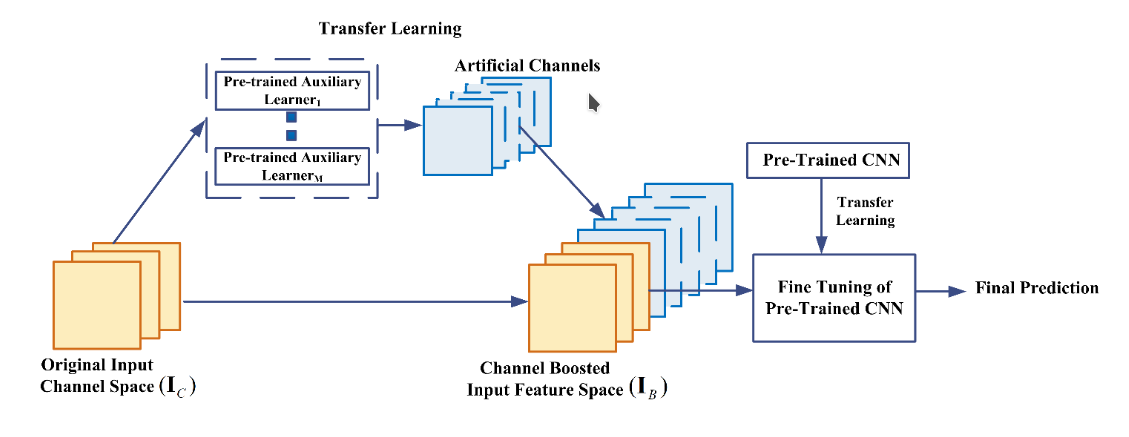
\includegraphics[scale=0.3]{content/channel_boosting.png}
    \caption{Channel Boosting}
    \label{fig:channel_boosting}
\end{figure}


\subsubsection{Attention based}
Their goal is to choose which patch is the most important area in an image. Focusing on these relevant features plays a significant role in image localization and recognition. This is true both for the channels but also spatially.

\textbf{Exemples}: Residual Attention Neural Network, Convolutional Block Attention Module

\section{Layers}
\subsection{Conv2d}
The spatial size of the input changes as follows:

\begin{equation}
    H_{out} = \left\lfloor \frac{H_{in}+2\times padding[0] - dilation[0]\times (kernel\_size[0]-1)-1}{stride[0]}+1 \right\rfloor
\end{equation}
\begin{equation}
    W_{out} = \left\lfloor \frac{W_{in}+2\times padding[1]-dilation[1]\times(kernel\_size[1]-1)-1}{stride[1]}+1 \right\rfloor
\end{equation}

\subsection{Softmax}
Applying Softmax rescales the element of a tensor so that they range in [0, 1] and sum to 1. The output of this layer is often interpreted as probabilities.
\begin{equation}
    Softmax(x_i) = \frac{exp(x_i)}{\sum_j exp(x_j)}
\end{equation}

\subsection{LogSoftmax}
Applying LogSoftmax additionally applies log to a softmax. The output can be interpreted as log-probabilities.
\begin{equation}
    LogSoftmax(x_i) = log\left(\frac{exp(x_i)}{\sum_j exp(x_j)}\right)
\end{equation}
\section{Loss Functions}

\subsection{L1 Loss}
It creates a criterion that measures the mean absolute error (MAE) between the input $x$ and the target $y$.
\begin{equation}
    L = \frac{1}{N} \sum_{i=0}^{N} = |x_i - y_i|
\end{equation}

\subsection{MSE Loss}
It creates a criterion that measures the mean squared error between the input $x$ and the target $y$.
\begin{equation}
    L =  \frac{1}{N} \sum_{i=0}^{N} = (x_i - y_i)^2
\end{equation}

\subsection{Cross-entropy Loss}
This loss function is used for classification. It combines the \textit{Log Softmax} and the \textit{NLL Loss} into a single loss. 
This criterion expects a class index $class$ as target value and the input $x$ should contain raw, unnormalized scores for each class.
\begin{equation}
    loss(x, class) = -\log \left(\frac{\exp(x_{class})}{\sum_j \exp(x_j)}\right)
\end{equation}
The losses are averaged across observations for each minibatch.
\begin{equation}
    L = \frac{1}{N} loss(x_i, class_i)
\end{equation}

\subsection{Negative Log-Likelihood Loss (NLL)}
 It is useful to train a classification problem with C classes.
 The input contains the log-probabilities of each class. These can be obtained from a \textit{LogSoftmax} layer.
 
 \begin{equation}
    l_n(x_n, y_n) = -x_{n, y_n} 
 \end{equation}
which is just the negative log-probability of the ground-truth class.
For a batch of size N, the total loss can be:
\begin{equation}
    L = \left\{ \begin{array}{ll}
        \frac{1}{N}\sum_{n=1}^{N} l_n &\;if\;reduction="mean" \\
        \sum_{n=1}^{N} l_n &\;if\;reduction="sum"
    \end{array}\right.
\end{equation}

Optionally, it is possible to specify weights $w_i$ to each class. The loss becomes
\begin{equation}
    l_n(x, y) = -w_{y_n} x_{n, y_n}
\end{equation}

\section{Brier score}
The Brier score is a \textbf{proper score function} that measures the accuracy of probabilistic predictions. It can be applied to tasks where the output is a set of probabilities corresponding to mutually-exclusive discrete outcomes.

It is defined as the \textit{mean squared error} between the predicted probabilities and the one-hot encoded ground-truth.

\begin{equation}
    Brier = \frac{1}{N}\sum_{t=1}^{N} (f_t - y_t)^2
\end{equation}

where $f_t$ is the probability predicted for the class $t$ and $y_t$ is either 0 or 1.


\section{Yolo}
Basic idea for the Yolo (v1, v2, v3) object detection algorithm.

\begin{algorithm}[H]
\DontPrintSemicolon
\KwInput{Input image}
\KwOutput{a set of bounding boxes with confidence and label}
 Divide the image in a $S\times S$ grid. \\
\For{each cell}
  { predict: \\
  - B boxes ($c_x, c_y, w, h$ for each anchor box) \\
  - B confidence values (the confidence should be equal to $Pr(Object) \times IoU$, if there is no object in the cell it should be 0 and if there is if should be equal to the IoU with its bbox) \\
  - C class conditional probabilities ($Pr(class_i|Object$) \\}
 The final tensor is $S\times S \times (B \times 5 + C)$ \\
 Threshold and apply non-maximum suppression
\caption{Yolo}
\end{algorithm}


\section{Mask R-CNN}
Basic idea for the Mask R-CNN object detection and segmentation

\begin{algorithm}[H]
\DontPrintSemicolon
\KwInput{Input image}
\KwOutput{a set of bounding boxes + label + mask}
 Apply the \textit{backbone} network to compute feature maps \\
 Apply the RPN (Region Proposal Network) that outputs candidate RoI (objectness scores + box coordinates) \\
 Apply Fast R-CNN on each RoI with an additional branch for the mask:\\
 \For{each RoI}
 {
  apply Fast R-CNN with an additional branch for the mask: \\
 - classification: a set of class scores  \\
 - bbox regression: per-class bbox offsets \\
 - mask prediction: one binary mask per class \tcp*{only the mask corresponding to the true class is used during training}
 }
 \caption{Mask R-CNN}
\end{algorithm}

\section{Automatic Differentiation}


Different methods can be used to compute gradients:
\begin{itemize}
    \item manually working out the derivative and coding them: complicated and very long to do
    \item \textit{numerically differentation} using finite difference approximation: unstable and expensive
    \item \textit{symbolic differentiation} using tools such as Maple or SymPy: limited to small functions because the size of the expression grows exponentially
    \item \textit{automatic differentiation}: much better
\end{itemize}



There are two ways to do Autodiff (AD): a forward mode and a reverse mode

\subsection{Forward Mode}

In the forward mode the derivative are passed from the input to the output. For example, if we want to compute the derivative wrt. $x_1$, we compute each intermediate derivative:

\begin{equation}
    \dot{v}_i = \frac{\delta v_i}{\delta x_1}
\end{equation}

This generalizes to compute the Jacobian of a function $f: \mathbb{R}^n \xrightarrow{} \mathbb{R}^m$.
To compute the derivative wrt. input $x_i$, we set its derivative to one $\dot{x}_i = 1$ and the derivative of all other inputs to $\dot{x}_{j(j \ne i)} = 0$. This can give a complete column of the Jacobian. To compute the full Jacobian $n$ passes are required.

Furthermore, forward mode AD is very efficient for Jacobian-vector product. In that case, we just need to set the input derivatives to $r$, as the final matrix-vector product is just a weigthed-sum of the Jacobian columns.

\begin{equation}
    \mathbf{J}_f r = \left[\begin{array}{ccc}
        \frac{\delta y_1}{\delta x_1} & \hdots & \frac{\delta y_1}{\delta x_n}  \\
        \vdots & \ddots & \vdots \\
        \frac{\delta y_m}{\delta x_1} & \hdots & \frac{\delta y_m}{\delta x_n}
    \end{array}\right]
    \left[\begin{array}{c}
        r_1 \\
        \vdots \\
        r_n 
    \end{array}\right]
\end{equation}

In conclusion, forward mode AD, is very useful for functions with a small numbers of inputs wrt. outputs.


\begin{figure}[H]
    \centering
    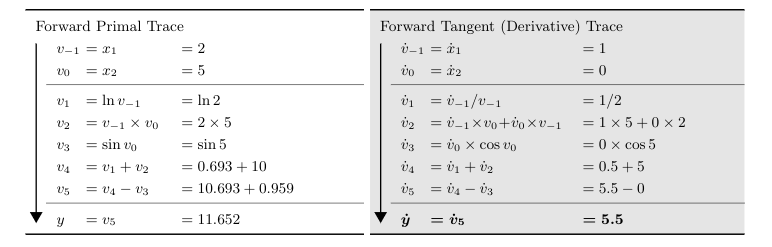
\includegraphics[scale=0.6]{content/Forward_AD_example.png}
    \caption{Forward AD of $y=f(x_1, x_2)=ln(x_1)+x_1x_2-sin(x_2)$ evaluated at $(x_1, x_2)=(2, 5)$. We set $\dot{x_1}=1$ and $\dot{x_2}=0$ to compute $\frac{\delta y}{\delta x_1}$}
    \label{fig:my_label}
\end{figure}


\subsubsection{Dual Numbers}
Mathematically, forward AD can be viewed as evaluating functions using dual numbers, which can be defined as truncated Taylor series of the form
\begin{equation}
    v + \dot{v}\epsilon
\end{equation}
where $v, \dot{v} \in \mathbb{R}$ and $\epsilon$ is a nilpotent number, such that $\epsilon^2 = 0$ and $\epsilon \ne 0$.

The idea is to use dual numbers as data structures for carrying the tangent value together with the primal.
The chain rules works as expected on this representation.


\subsection{Reverse Mode}

Reverse mode propagates derivated backward from the outputs to the inputs. This is done by complementing each intermediat variable $v_i$ with an adjoint
\begin{equation}
    \bar{v_i} = \frac{\delta y_j}{\delta v_i}
\end{equation}
which represents the sensitivity of a considered output $y_j$ wrt. the changes in $v_i$.

In a first phase, a forward pass is done to compute the intermediate variables $v_i$ and record the dependencies in the computational graph through a book-keeping procedure.
Then, the chain rule is used for back-propagating the derivatives.


In this mode, computing the derivative of an output wrt. each input is done in one pass. This is much better than the forward mode. However, a new pass is required for each output.

Similarly to the forward mode, the reverse mode can be used to compute the transpose Jacobian-vector product directly by setting $\bar{y} = r$.

\begin{equation}
    \mathbf{J}_f^T r = \left[\begin{array}{ccc}
        \frac{\delta y_1}{\delta x_1} & \hdots & \frac{\delta y_m}{\delta x_1}  \\
        \vdots & \ddots & \vdots \\
        \frac{\delta y_1}{\delta x_n} & \hdots & \frac{\delta y_m}{\delta x_n}
    \end{array}\right]
    \left[\begin{array}{c}
        r_1 \\
        \vdots \\
        r_m
    \end{array}\right]
\end{equation}



In conclusion, reverse mode AD is more efficient when the number of inputs is larger than the number of outputs.

This is why it is the solution used in neural network, where $n$ is usually large and $m=1$.